\section{Partie 2}

\subsection{Statistiques}

\begin{table}[H]
    \centering
    \begin{tabular}{|l|c|c|}
        \hline
        \textbf{Type}  & \textbf{\# trouvées par SOLInspect} & \textbf{\# trouvées manuellement} \\ \hline
        SELECT         & 18                                  & 24                                \\ \hline
        UPDATE         & 4                                   & 24                                \\ \hline
        DELETE         & 2                                   & 27                                \\ \hline
        INSERT         & 5                                   & 16                                \\ \hline
        CREATE TABLE   & 18                                  & 18                                \\ \hline
        CREATE INDEX   & 8                                   & 8                                 \\ \hline
        ALTER TABLE    & 24                                  & 24                                \\ \hline
        \textbf{Total} & \textbf{79}                         & \textbf{141}                      \\ \hline
    \end{tabular}
    \caption{Nombre de requêtes trouvées par type.}
\end{table}

Pour les requêtes de la colonne « \# trouvées manuellement », un script \texttt{Python} a été utilisé pour effectuer une analyse statique des requêtes. Il permet de parcourir les différents fichiers Java et, grâce à une regex, les différents appels à SQLite tels que \mintinline{java}{db.update} ou encore \mintinline{java}{db.execSQL} sont filtrés et enregistrés dans des fichiers séparés.

Pour la complexité de ces dernières, elles sont plutôt simples et courtes. On notera toutefois que les requêtes de création de table peuvent être plus longues, notamment pour la table \mintinline{java}{presets}, mais restent, malgré tout, simples à interpréter.

À propos de la répartition des requêtes dans le projet, elles sont regroupées dans 12 fichiers Java différents. Ces 12 fichiers sont répartis parmi 7 dossiers alors que le projet en compte 58.

\begin{table}[H]
    \centering
    \begin{tabular}{|l|l|}
        \hline
        \textbf{Dossier}                                     & \textbf{Fichier}                           \\ \hline
        \texttt{src/main/java/de/blau/android/filter}        & \texttt{TagFilterActivity.java}            \\
                                                             & \texttt{TagFilterDatabaseHelper.java}      \\ \hline
        \texttt{src/main/java/de/blau/android/imageryoffset} & \texttt{ImageryOffsetDatabase.java}        \\ \hline
        \texttt{src/main/java/de/blau/android/photos}        & \texttt{PhotoIndex.java}                   \\ \hline
        \texttt{src/main/java/de/blau/android/prefs}         & \texttt{AdvancedPrefDatabase.java}         \\ \hline
        \texttt{src/main/java/de/blau/android/resources}     & \texttt{KeyDatabaseHelper.java}            \\
                                                             & \texttt{TileLayerDatabase.java}            \\ \hline
        \texttt{src/main/java/de/blau/android/services/util} & \texttt{MapTileProviderDataBase.java}      \\
                                                             & \texttt{MBTileProviderDataBase.java}       \\ \hline
        \texttt{src/main/java/de/blau/android/validation}    & \texttt{ValidatorRulesDatabase.java}       \\
                                                             & \texttt{ValidatorRulesDatabaseHelper.java} \\
                                                             & \texttt{ValidatorRulesUI.java}             \\ \hline
    \end{tabular}
    \caption{Répartition des fichiers contenant des requêtes SQL.}
\end{table}

\newpage
\subsection{Répartition du type de requêtes par tables}
\begin{figure}[!ht]
    \centering
    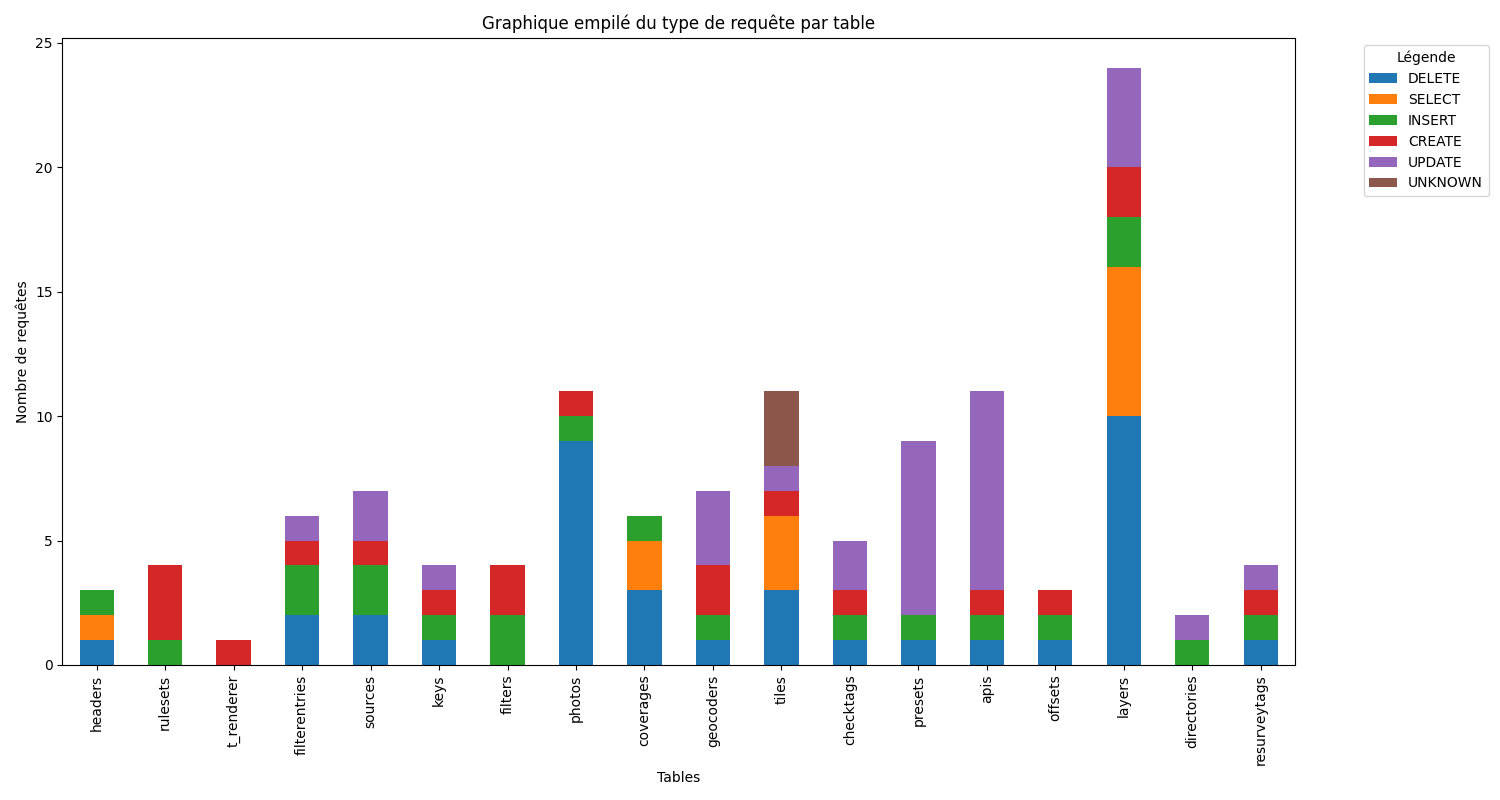
\includegraphics[scale=0.5]{images/stats.png}
    \label{fig:Statistiques du nombre de requête par table}
\end{figure}

\newpage
\subsection{Sous-schéma logique}
\begin{figure}[!ht]
    \centering
    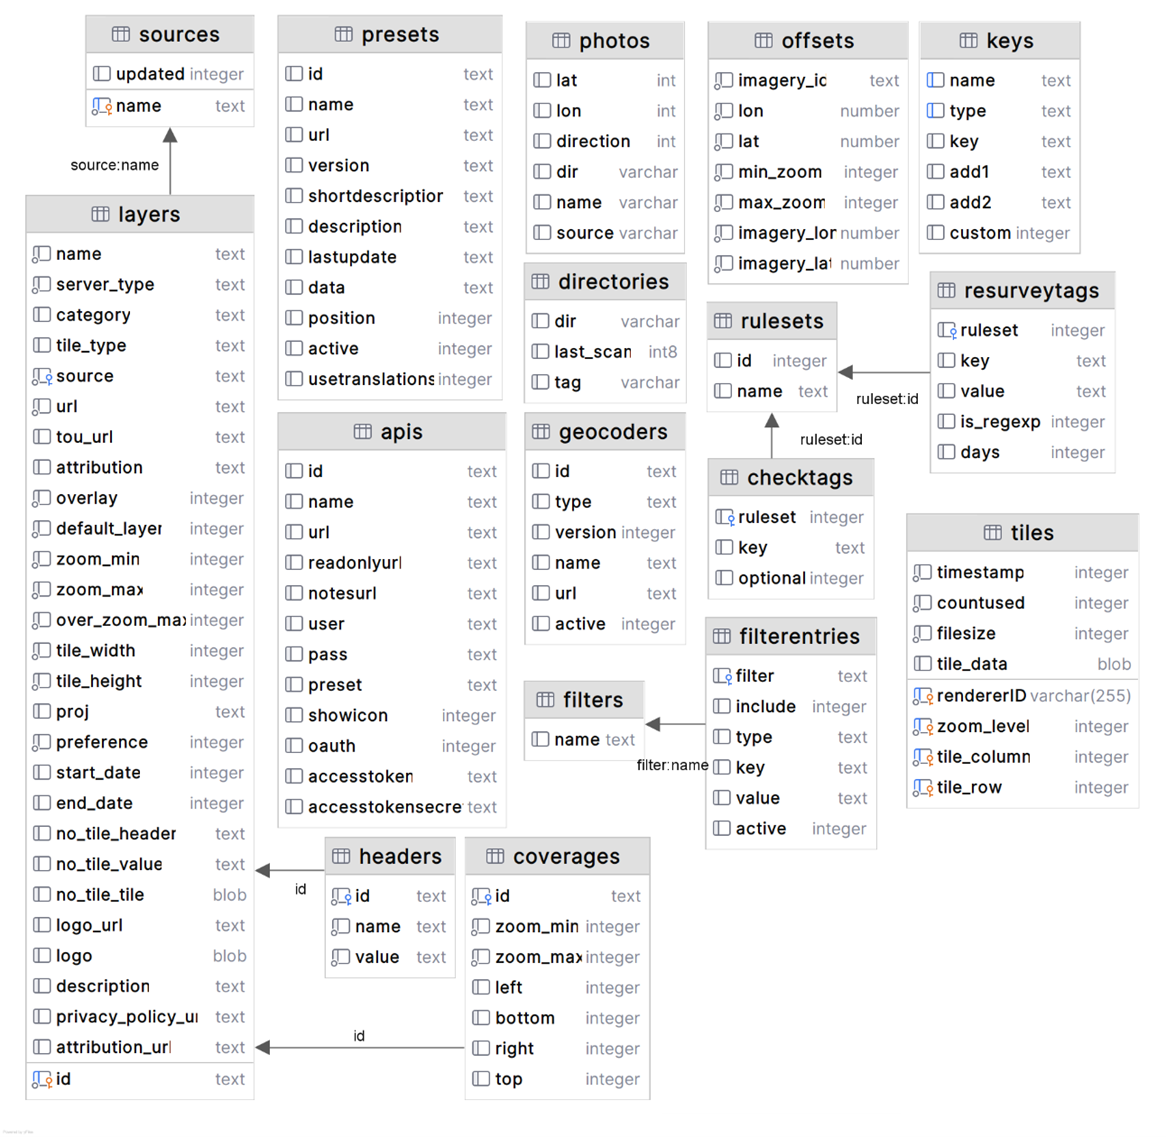
\includegraphics[scale=1]{images/sous_schema_logique.png}
    \label{fig:sous schéma logique}
\end{figure}
